\documentclass[tikz,border=2pt]{standalone}
\usepackage{amsmath,amssymb}
\usepackage{tikz}
\usetikzlibrary{arrows.meta}

\begin{document}
% Giapetto feasible region (finishing 2 x_s + x_t <= 100, carpentry x_s + x_t <= 80,
% soldier demand x_s <= 40). With objective 2 x_s + 2 x_t the objective lines are parallel
% to the carpentry edge x_s + x_t = 80: every point of that edge, from (0,80) to (20,60),
% is optimal with z = 160; the dashed line is the level z = 100.
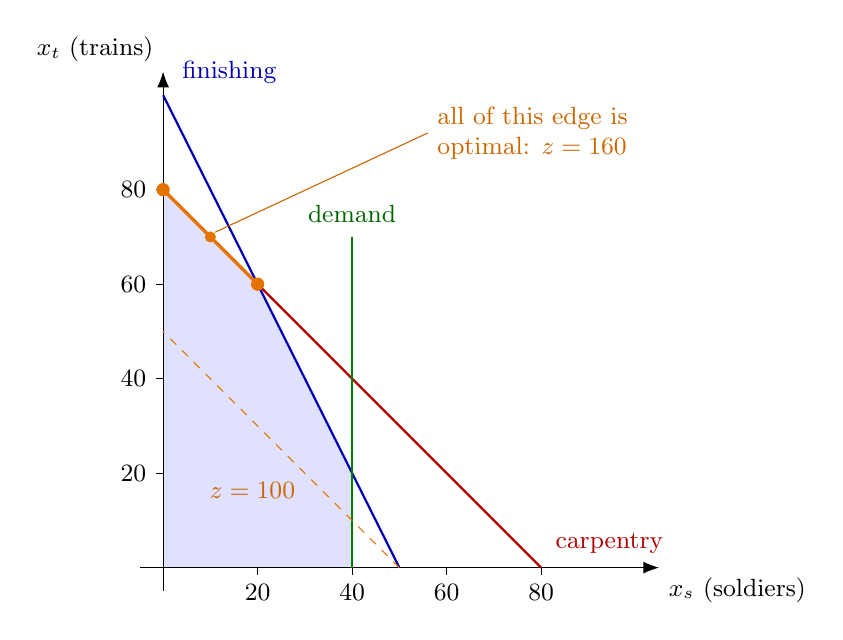
\begin{tikzpicture}[x=0.06cm, y=0.06cm, every node/.style={font=\small}, >={Latex[length=2mm]}]
	\fill[blue!12] (0,0) -- (40,0) -- (40,20) -- (20,60) -- (0,80) -- cycle;
	\draw[->] (-5,0) -- (105,0) node[below right] {$x_s$ (soldiers)};
	\draw[->] (0,-5) -- (0,105) node[above left] {$x_t$ (trains)};
	\foreach \t in {20,40,60,80} {
		\draw (\t,0) -- (\t,-1.5) node[below] {$\t$};
		\draw (0,\t) -- (-1.5,\t) node[left] {$\t$};
	}
	\draw[blue!70!black, thick] (50,0) -- (0,100);
	\draw[red!70!black, thick] (80,0) -- (0,80);
	\draw[green!50!black, thick] (40,0) -- (40,70);
	\node[blue!70!black, anchor=south west] at (2,100.5) {finishing};
	\node[red!70!black, anchor=south west] at (81,1) {carpentry};
	\node[green!40!black, anchor=south] at (40,71) {demand};
	\draw[orange!90!black, dashed] (50,0) -- (0,50) node[pos=0.4, anchor=north east, orange!80!black] {$z=100$};
	\draw[orange!90!black, very thick] (0,80) -- (20,60);
	\fill[orange!90!black] (0,80) circle (2.4pt);
	\fill[orange!90!black] (20,60) circle (2.4pt);
	\fill[orange!90!black] (10,70) circle (2pt);
	\draw[orange!80!black, thin] (11,71) -- (56,92);
	\node[orange!80!black, anchor=west, align=left] at (56,92) {all of this edge is\\ optimal: $z=160$};
	\end{tikzpicture}
\end{document}
